\def \projectname{STAKEPOOL\xspace}

\def \company{POS Mining CO}
\def \companyref{N/A}
\def \companytype{OTHER SMALL BUSINESS}
\def \team{N/A}
\def \restrictions{Proprietary Information}
\def \title{\projectname}
\def \biline{Proof Of Stake Mining Cryptocurrency}
\def \author{Your Name}
\def \email{stakepool@stakepool.co}
\def \phone{http://stakepool.co}
\def \address{Ontario, CA}

%%
% for each of the following items, uncommenting the fields will make them show up in the appropriate places
%% 

\def \placeofperformance{\address}
%\def \classification{For Official Use Only}   % only define if this is classified
%\def \exportcontrol{} % uncomment if this document is export controlled
%\def \proposalcontrol{} % uncomment if this is a proposal with restricted release for .gov purposes

%% the following are only needed for proposals.  
\def \baa{Whitepaper}
\def \techarea{Technical Area 1 (Your mom's tech area)}
\def \doctitle{Volume I (Technical and Management Proposal)}
\def \cost{\$1,000,000}

\def \duns{111111111}
\def \cagecode{222222}
\def \tin{33-3333333}
\def \awardtype{Cost Plus Fixed Fee (CPFF)}
\def \pop{January 1, 2000 - December 31, 2020 (3 days)}
\def \submitdate{January 1, 2020}

\documentclass[letterpaper,12pt]{article}

\usepackage[printonlyused]{acronym}
\usepackage{amsmath}
\usepackage[font={small,sf},labelfont={small,sf}]{caption}
\usepackage{color}
\usepackage{fancyhdr}
\usepackage[includeheadfoot,left=1in,top=.4in,right=1in,bottom=.75in,headsep=\dimexpr3cm-59pt\relax,headheight=59pt]{geometry}
\usepackage{graphicx}
\usepackage[pagebackref,hyperindex=true]{hyperref}
\usepackage{listings}
\usepackage{longtable}
\usepackage{mdwlist}
\usepackage{parskip}
\usepackage{setspace}
\usepackage{tabularx}
\usepackage[compact]{titlesec}
\usepackage{xfrac}
\usepackage{xspace}
\usepackage{tikz}
\usetikzlibrary{calc,matrix}
\usepackage{charter}
\usepackage{environ}
\usepackage{hyperref}

% default font packages
\usepackage{courier} % use courier for the mono-spaced font 
\usepackage{helvet}  % use a Helvetica clone for default text (sans-serif)

%%%
% default document settings
%%%

% setup the default fonts for section headers
\titleformat*{\section}{\sffamily\fontsize{16}{16}\selectfont\bfseries}
\titleformat*{\subsection}{\sffamily\fontsize{14}{14}\selectfont\bfseries}
\titleformat*{\subsubsection}{\sffamily\fontsize{12}{12}\selectfont\bfseries}
\titleformat*{\paragraph}{\sffamily\fontsize{12}{12}\selectfont\bfseries}
\titleformat*{\subparagraph}{\sffamily\fontsize{12}{12}\selectfont\bfseries}

% section numbering
\setcounter{tocdepth}{3}     % display only 3 sections deep in the table of contents
\setcounter{secnumdepth}{5}  % number to 5 sections deep

% add acronyms to the TOC (use chapter, if chapters are available, otherwise use sections
% Based off of suggestions at: http://jevopi.blogspot.com/2009/09/acronyms-and-latex.html
\providecommand{\listofacronymsname}{List of Acronyms}
\providecommand{\listofacronyms}{
    \ifx\chapter\undefined
        \chapter*{\listofacronymsname}
	    % \addcontentsline{toc}{chapter}{\listofacronymsname}
    \else
        \section*{\listofacronymsname}
		% \addcontentsline{toc}{section}{\listofacronymsname}
    \fi
    \label{sec:acronyms}
	\markboth{\listofacronymsname}{\listofacronymsname}
    \begin{acronym}[AAAAAAAAAAA]
\acro{POS}{Proof-Of-Stake}
\end{acronym}

}


%%%
% custom page styles
%%%

\fancypagestyle{restricted}{
    \fancyhead[L]{\rule[-2ex]{0pt}{2ex}\small \MakeUppercase{\baa}}
    \fancyhead[c]{ 
        \small
        \ifdefined\classification
        \textbf{\classification} \\ 
        \fi
        \textbf{ \company } \\
%        \textbf{\MakeUppercase{\restrictions} } \\
        \title{}: \biline
    }
    \fancyhead[R]{\small \MakeUppercase{\baa}}

    \fancyfoot[L]{\small \title}
%    \fancyfoot[c]{\small \textbf{{\MakeUppercase{\restrictions}}}}
    \fancyfoot[c]{
        \small
%        \textbf{\MakeUppercase{\restrictions} } \\
        \ifdefined\classification
        \textbf{\classification}
        \fi
    }
    \fancyfoot[R]{\small \thepage}
}

\fancypagestyle{plain}{
    \fancyhead[L]{\rule[-2ex]{0pt}{2ex}\small \MakeUppercase{\baa}}
    \fancyhead[C]{ 
        \small
        \ifdefined\classification
        \textbf{\classification} \\ 
        \fi
        \textbf{ \company } \\
        \title{}: \biline
    }
    \fancyhead[R]{\small \MakeUppercase{\baa}}

    \fancyfoot[L]{\small \title}
    \fancyfoot[C]{
        \small
        \ifdefined\classification
        \textbf{\classification}
        \fi
    }
    \fancyfoot[R]{\small \thepage}
}

% set the default page style to "plain"
\pagestyle{plain}

%%%
% page templates
%%%

\newcommand{\whitepapercover}{
    \begin{titlepage}
    \thispagestyle{empty}
    \vspace*{1.25in}

    \hfill \textsc{\sffamily\huge\bfseries \title} \\
    \begin{flushright}
        \textsc{\sffamily\large \biline} \\
        \textsc{\sffamily\large \today}
    \end{flushright}

    \vspace{1.0in}
    \begin{center}
        
\includegraphics[width=4.0in]{includes/logo.png}
    \end{center}

    \end{titlepage}
    \cleardoublepage
}

\newcommand{\proposalcover}{
    \thispagestyle{empty}
    \vspace*{-1.25in}
    \begin{center}
        
\includegraphics[width=4.0in]{includes/logo.png}
    \end{center}
  
    {
        \footnotesize
        \begin{center}
	        \begin{tabular}{|l|p{3.5in}|}
	            \hline
	            \textbf{BAA Number} & \baa \\ \hline
	            \textbf{Technical Area} & \techarea \\ \hline
	            \textbf{Lead Organization} & \company \\ \hline
                
                \ifdefined\companytype
	            \textbf{Type of Business} & \companytype \\ \hline
                \fi

                \ifdefined\companyref
	            \textbf{Contractor's Reference Number} & N/A \\ \hline
                \fi

                \ifdefined\team
	            \textbf{Team Members} & \team \\ \hline
                \fi

	            \textbf{Proposal Title} & \title : \biline \\ \hline
	            \textbf{Technical Point of Contact} & \author \\ & \email \\ & \phone \\ & \address \\ \hline
	            \textbf{Administrative Point of Contact} & \author \\ & \email \\ & \phone \\ & \address \\ \hline

                \ifdefined\cost
	            \textbf{Proposed Cost} & \cost \\ \hline
                \fi

                \ifdefined\submitdate
	            \textbf{Date Submitted} & \submitdate \\ \hline
                \fi

                \ifdefined\awardtype
	            \textbf{Award Instrument Requested} & \awardtype \\ \hline
                \fi

                \ifdefined\placeofperformance
	            \textbf{Place of Performance} & \placeofperformance \\ \hline
                \fi

                \ifdefined\pop
	            \textbf{Period of Performance}  & \pop \\ \hline
                \fi

	            \textbf{Date Prepared} & \today \\ \hline

                \ifdefined\duns
	            \textbf{DUNS Number} & \duns \\ \hline
                \fi

                \ifdefined\tins
	            \textbf{TIN number} & \tin \\ \hline
                \fi
                
                \ifdefined\cagecode
	            \textbf{Cage Code} & \cagecode \\ \hline
                \fi
	            \textbf{Proposal Validity Period} & This proposal is valid for 120 days \\ \hline
	        \end{tabular}
        \end{center}
    }

    \ifdefined\proposalcontrol
    \section*{Use and Disclosure of Data}
    This proposal includes data that shall not be disclosed outside the Government and shall not be duplicated, used, or disclosed—in whole or in part - for any purpose other than to evaluate this response.  If, however, a contract is awarded to this offeror as a result of - or in connection with - the submission of this data, the Government shall have the right to duplicate, use, or disclose the data to the extent provided in the resulting contract.  This restriction does not limit the Government's right to use information contained in this data if it is obtained from another source without restriction.
    \fi
    \cleardoublepage
}

\newcommand{\bib}{
    \cleardoublepage
    \pagestyle{plain}
    \phantomsection
    \ifx\chapter\undefined
        \addcontentsline{toc}{chapter}{References}
    \else
        \addcontentsline{toc}{section}{References}
    \fi
    \bibliographystyle{unsrt} % unsrt = plain, except sorted by use, not date.
    {
        \raggedright
        \bibliography{includes/refs}
    }
}

\newcommand{\docinfo}{
    \pagenumbering{roman}
    \thispagestyle{plain}
    \section*{Copyright}
    Copyright \copyright \the\year \xspace \company.

    All trademarks within this document belong to their respective owners.

    \section*{Authors}
    \author, \company

    \section*{Point of Contact}
            
    \author \\ \email \\ \phone 
    
    \ifdefined\exportcontrol
    \section*{Export Control}
    WARNING - This document contains Technical Data whose export is restricted by the Arms Export Control Act (Title 22, U.S.C., Sec 2751, et seq.).  Violations of these export laws are subject to severe criminal penalties.
    \fi
    
    \cleardoublepage

    \tableofcontents
    \listoftables
    \listoffigures
    \listofacronyms 
    \cleardoublepage
    \pagenumbering{arabic}
}

%%%
% ease of use macros
%%%

% Example: \q{foo} 
% Results: "foo" - except the quote marks go the right way.
\newenvironment{q}[1]{``#1''} 

% example: C:$\bs$Program Files$\bs$Adobe$\bs$
% Results: C:\Program Files\Adobe\
\def \bs{\char`\\}

% example: \begin{fig}{figure label}{figure caption}{ ... }
% results: A figure, boxed in the center, with font slightly shrunk, with a label and caption
\newcommand{\temporarylabel}{}
\newcommand{\temporarycaption}{}
\newenvironment{fig}[2]{
    \renewcommand{\temporarylabel}{#1}
    \renewcommand{\temporarycaption}{#2}
    \begin{figure}[!htbp]
    \begin{center}
    \begin{small}
}{
    \end{small}
    \end{center}
    \caption{\temporarycaption \label{\temporarylabel}}
    \end{figure}
}


% code by Andrew:
% http://tex.stackexchange.com/a/28452/13304
\makeatletter
\let\matamp=&
\catcode`\&=13
\makeatletter
\def&{\iftikz@is@matrix
  \pgfmatrixnextcell
  \else
  \matamp
  \fi}
\makeatother

\newcounter{lines}
\def\endlr{\stepcounter{lines}\\}

\newcounter{vtml}
\setcounter{vtml}{0}

\newif\ifvtimelinetitle
\newif\ifvtimebottomline
\tikzset{description/.style={
  column 2/.append style={#1}
 },
 timeline color/.store in=\vtmlcolor,
 timeline color=red!80!black,
 timeline color st/.style={fill=\vtmlcolor,draw=\vtmlcolor},
 use timeline header/.is if=vtimelinetitle,
 use timeline header=false,
 add bottom line/.is if=vtimebottomline,
 add bottom line=false,
 timeline title/.store in=\vtimelinetitle,
 timeline title={},
 line offset/.store in=\lineoffset,
 line offset=4pt,
}

\NewEnviron{vtimeline}[1][]{%
\setcounter{lines}{1}%
\stepcounter{vtml}%
\begin{tikzpicture}[column 1/.style={anchor=east},
 column 2/.style={anchor=west},
 text depth=0pt,text height=1ex,
 row sep=1ex,
 column sep=1em,
 #1
]
\matrix(vtimeline\thevtml)[matrix of nodes]{\BODY};
\pgfmathtruncatemacro\endmtx{\thelines-1}
\path[timeline color st] 
($(vtimeline\thevtml-1-1.north east)!0.5!(vtimeline\thevtml-1-2.north west)$)--
($(vtimeline\thevtml-\endmtx-1.south east)!0.5!(vtimeline\thevtml-\endmtx-2.south west)$);
\foreach \x in {1,...,\endmtx}{
 \node[circle,timeline color st, inner sep=0.15pt, draw=white, thick] 
 (vtimeline\thevtml-c-\x) at 
 ($(vtimeline\thevtml-\x-1.east)!0.5!(vtimeline\thevtml-\x-2.west)$){};
 \draw[timeline color st](vtimeline\thevtml-c-\x.west)--++(-3pt,0);
 }
 \ifvtimelinetitle%
  \draw[timeline color st]([yshift=\lineoffset]vtimeline\thevtml.north west)--
  ([yshift=\lineoffset]vtimeline\thevtml.north east);
  \node[anchor=west,yshift=16pt,font=\large]
   at (vtimeline\thevtml-1-1.north west) 
   {\textsc{Timeline \thevtml}: \textit{\vtimelinetitle}};
 \else%
  \relax%
 \fi%
 \ifvtimebottomline%
   \draw[timeline color st]([yshift=-\lineoffset]vtimeline\thevtml.south west)--
  ([yshift=-\lineoffset]vtimeline\thevtml.south east);
 \else%
   \relax%
 \fi%
\end{tikzpicture}
}


\usepackage[utf8]{inputenc}
\usepackage[cyr]{aeguill}
\usepackage[francais]{babel}

\begin{document}

\shorthandoff{:!}

\def\angle{0}
\def\radius{3}
\def\cyclelist{{"orange","blue","red","green"}}
\newcount\cyclecount \cyclecount=-1
\newcount\ind \ind=-1


\whitepapercover
%\docinfo

% mark pages that have restricted (aka: proprietary information with the "restricted" page style.
%\pagestyle{restricted}


\begin{abstract}
StakePool (POOL) est un jeton Ethereum ERC-20 qui représente un droit aux bénéfices tirés de la puissance de minage par preuve d'enjeu (Proof Of Stake, POS) de l'infrastructure de StakePool.co. Le réseau StakePool.co utilise la preuve d'enjeu (POS) sur plusieurs types de masternodes pour maximiser le retour sur investissement. Le jeton sera disponible durant la levée de fond (ICO) qui durera 60 jours. Durant la première vague, 50 millions de jetons au maximum seront vendus. Durant la deuxième vague, 100 millions seront vendus, puisque de plus en plus de crypto-monnaies migreront vers la preuve d'enjeu, dont l'Ethereum. Cette deuxième vague aura lieu entre 60 et 90 jours avant la bascule d'Ethereum vers la preuve d'enjeu (mise à jour Casper). Les jetons restants seront gardés de côté pour d'éventuels d'autres migrations vers la preuve d'enjeu ou masternodes. Une troisième vague n'aura lieu plus tard qu'en cas de besoin d'investissements supplémentaires. Dans le cas contraire, les jetons restants seront brûlés.
	
\end{abstract}

\section{The StakePool project}

Qu'est ce que StakePool : Le projet StakePool, issu d'une société américaine (POS Mining Co.) basée en Ontario (Canada), maintient des portefeuilles POS et des masternodes pour les crypto-monnaies à preuve d'enjeu (POS). 25\% de notre approvisionnement en éléctricité est issu de l'énergie solaire. Chaque jeton POOL représente un pourcentage des profits générés par le minage, et est payé mensuellement en ETH, directement dans le portefeuille des détenteurs de jetons. Comme pour la plupart des jetons, les jetons POOL devraient être listés sur plusieurs place d'échange.

\textbf{\emph{La philosophie de la preuve d'enjeu est non pas ``la sécurité vient de l'énergie dépensée'', mais plutôt ``la sécurité vient de l'immobilisation d'un bien économique''.}}  \cite{vbuterinposphi}

 \subsection{Notre vision}
  \subsubsection{Histoire du projet}
Les fondateurs de StakePool ont maintenu des portefeuilles POS et des masternodes pour plusieurs clients depuis plus de deux ans maintenant. En commençant par DASH, Blackcoin, Diamond, NEM et Reddcoin, puis avec OkCoin, Stratis et Decred, ils ont commencé à regrouper les «coins» de leurs amis, leur famille, et de personnes rencontrés sur le net, afin d'augmenter les chances de récompenses. Comme les fonds continuaient à croître, ils ont commencé à miner de plus en plus de crypto-monnaies. Contrairement à la preuve de travail (Proof of Work, POW), l'investissement est entièrement sur la monnaie. Les coûts électriques et de matériel restent minimes.

  \subsubsection{Sécurité}
Le minage par preuve d'enjeu (POS) a ses propres challenges de sécurité. Pour le minage par preuve de travail (POW), les «coins» peuvent être stockées hors ligne dans un portefeuille papier ou matériel pour les protégér du vol. Pour le minage par preuve d'enjeu, les «coins» doivent être en ligne sur un portefeuille non verrouillé. StakePool a mis en place différentes mesures de sécurité physiques et logicielles pour éviter les intrusions. StakePool utilise un solution professionnelle d'atténuation d'attaque pas déni de service (DDOS).
  
  \subsubsection{Transparence}
Nous nous efforcerons d'être aussi transparents que possible, tout en gardant la sécurité comme premier objectif. À partir du 1er novembre, les adresses des pourtefeuilles seront postées en ligne, aussi bien pour les preuve d'enjeu (POS) que pour les masternodes.


 \subsection{Aspects techniques}
  \subsubsection{Pourquoi la preuve d'enjeu (POS) ?}
En 2015, la quantité d'électricité nécessaire au minage d'un bloc Bitcoin aurait suffit à alimenter 1,6 maison états-unienne pendant un jour. En 2016, c'était 2,5 maisons par bloc. Dans un papier récent, des chercheurs ont estimé que les transactions Bitcoin consommeront autant d'électricité que le Danemark d'ici 2020. Alors que l'adoption des crypto-monnaies s'accélère, c'est tout à fait contraire aux objectifs écologiques indispensables à notre planète

Les développeurs d'Ethereum se sont sentis concernés par ce problème et ont présenté une méthode de consensus plus écologique, qui avec la mise à jour vers la version Casper, migrera de la preuve de travail (POW) vers la preuve d'enjeu (POW).
 Ethereum rejoindra alors les nombreuses autres crypto-monnaies qui utilisent déjà la preuve d'enjeu (POS) depuis 2012.

La preuve d'enjeu n'est pas seulement un système plus juste, il est aussi des milliers de fois moins coûteux. Les propriétaires laissent simplement leurs «coins» sur leur portefeuille sur le réseau afin qu'ils maturent. Les investisseurs qui immobilisent ainsi leur «coins» peuvent gagner des récompenses — un peu comme s'il engrangaient des intérêts de leurs avoirs. La preuve d'enjeu ne requérant donc pas de matériel spécifique de minage (GPU,…), elle est plus juste, plus écologique, et évite une centralisation du minage, dangereuse pour le réseau.

\textbf{\emph{However, there is one SHA256 alternative that is already here, and that essentially does away with the computational waste of proof of work entirely: proof of stake. Rather than requiring the prover to perform a certain amount of computational work, a proof of stake system requires the prover to show ownership of a certain amount of money.}} \cite{vbuterin2013}

  \subsubsection{Qu'est ce que la preuve d'enjeu (POS)}
Le concept de la preuve d'enjeu (POS) repose sur le fait qu'une personne peut valider un bloc en fonction du nombre de «coins» dans son portefeuille. Plus on a de «coins», plus on a de puissance de minage. Le principe du minage par preuve d'enjeu est de garder les «coins» sur un portefeuille ouvert sur le réseau (donc pas sur un portefeuille matériel). Les portefeuilles forment ainsi un résau P2P, au travers duquel les transactions sont confirmées, et les récompenses correspondantes accordées. Ces récompenses sont les dividendes qui seront reversés au détenteurs de jetons POOL tous les mois.

\begin{figure}[h]
\centering
\caption{POW vs POS \cite{blockgeek}}
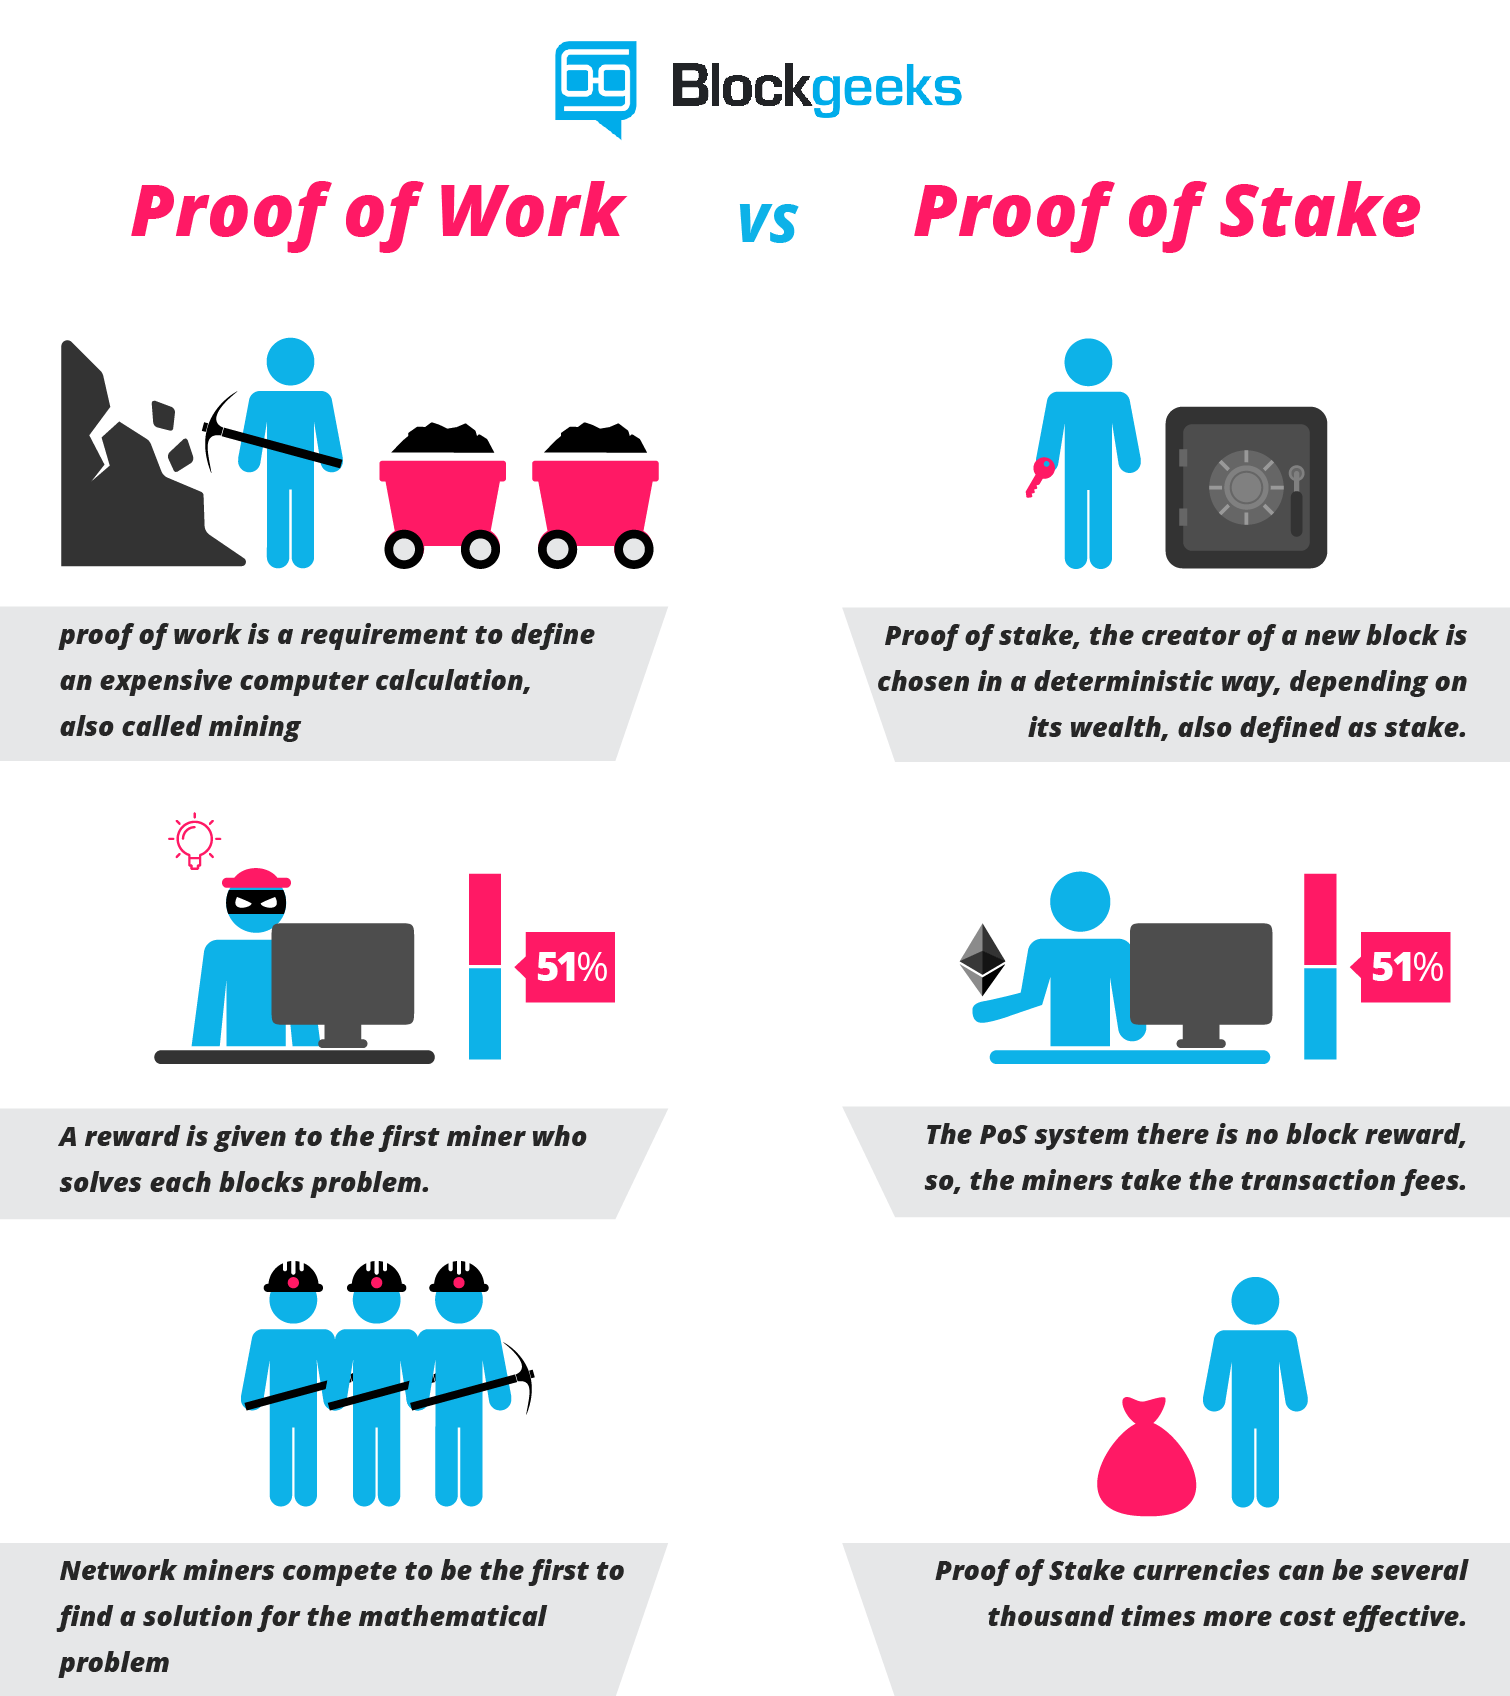
\includegraphics[width=10cm]{blockgeek.png}
\end{figure}

\subsubsection{Masternodes}
On peut le voir comme un serveur spécial, qui est maintenu en ligne 24h/24h. Les masternodes n'ont pas besoin de tiers de confiance, et sont décentralisés, à la manière des nœuds du réseau Bitcoin. Il y a quand même une différence majeure, puisque les masternodes Dash prennent part au protocole d'anonymisation Darksend. Les utilisateurs peuvent choisir d'envoyer des transactions anonymes directement depuis leur portefeuille Dash.

Chaque masternodes du réseau fourni un service d'anonymisation, s'assurant ainsi qu'il n'y a pas de point centralisé à attaquer ou à faire tomber. De plus, les masternodes assurent que les transactions sont validées en quasi temps-réel. Enfin, les opérateurs des masternodes Dash reçoivent une compensation financière pour le service rendu.

\newpage

\section{Émission des jetons}
Les jetons POOL seront émis pendant une phase de pre-ICO pour les premiers investisseurs. Tous les fonds levés lors de la phase de pre-ICO seront utilisés pour acheter des «coins» POS. Un bonus de 10% sera appliqué pour les jetons acquis pendant cette phase.

La première vague de la levée de fond officielle ne commencera qu'une fois le premier paiement au détenteurs des jetons pre-ICO effectué. Elle durera deux mois. Les ethereum collectés durant la première phase seront là aussi consacré à l'achat de nouveaux «coins» à preuve d'enjeu. Cependant, 10% seront consacrés à une réserve de fonds afin d'anticiper de nouvelles opportunités.

La seconde phase sera annoncée plus tard et sera consacrée à l'achat d'ETH pour préparer la bascule vers Casper.


\begin{figure}[h]
\centering
\caption{Distribution des jetons}
\begin{tikzpicture}[nodes = {font=\sffamily}]
	\foreach \percent/\name in {
		25/ICO  Round 1,
		50/ICO  Round 2,
		12.5/ICO  Round 3 (ou brûlés),
		12.5/Founders (blocqués pour deux ans)
	} {
		  \ifx\percent\empty\else               % If \percent is empty, do nothing
		  \global\advance\cyclecount by 1     % Advance cyclecount
		  \global\advance\ind by 1            % Advance list index
		  \ifnum3<\cyclecount                 % If cyclecount is larger than list
		  \global\cyclecount=0              %   reset cyclecount and
		  \global\ind=0                     %   reset list index
		  \fi
		  \pgfmathparse{\cyclelist[\the\ind]} % Get color from cycle list
		  \edef\color{\pgfmathresult}         %   and store as \color
		    % Draw angle and set labels
		  \draw[fill={\color!50},draw={\color}] (0,0) -- (\angle:\radius)
		  arc (\angle:\angle+\percent*3.6:\radius) -- cycle;
		  \node at (\angle+0.5*\percent*3.6:0.7*\radius) {\percent\,\%};
		  \node[pin=\angle+0.5*\percent*3.6:\name]
		  at (\angle+0.5*\percent*3.6:\radius) {};
		  \pgfmathparse{\angle+\percent*3.6}  % Advance angle
		  \xdef\angle{\pgfmathresult}         %   and store in \angle
		  \fi
	  };
\end{tikzpicture}
\end{figure}

\newpage

\section{Paiements}
La dernière semaine de chaque mois, une annonce rappellera à tous les détenteurs de jetons de garder leur jetons POOL dans un portefeuille Ethereum et non sur une place d'échange. En début de mois suivant, une feuille de calcul Google Docs sera publiée et annoncée. Elle contiendra la liste des détenteurs à la date butoir, et le montant d'ETH distribué à chacun. Le paiment interviendra aux alentours du 10 du mois. Les profits seront répartis comme suit : 65\% iront aux détenteurs de jetons, 25\% seront réinvestis pour acheter plus de «coins» POS, et 10\% couvreront les coûts opérationnels, les mises à niveau matériel, etc…

\begin{figure}[h]
\centering
\caption{Distribution des dividendes}
\begin{tikzpicture}[nodes = {font=\sffamily}]
	\foreach \percent/\name in {
		65/Détenteurs des jetons,
		25/Investissements,
		10/Couverture des frais,
	} {
		  \ifx\percent\empty\else               % If \percent is empty, do nothing
		  \global\advance\cyclecount by 1     % Advance cyclecount
		  \global\advance\ind by 1            % Advance list index
		  \ifnum3<\cyclecount                 % If cyclecount is larger than list
		  \global\cyclecount=0              %   reset cyclecount and
		  \global\ind=0                     %   reset list index
		  \fi
		  \pgfmathparse{\cyclelist[\the\ind]} % Get color from cycle list
		  \edef\color{\pgfmathresult}         %   and store as \color
		    % Draw angle and set labels
		  \draw[fill={\color!50},draw={\color}] (0,0) -- (\angle:\radius)
		  arc (\angle:\angle+\percent*3.6:\radius) -- cycle;
		  \node at (\angle+0.5*\percent*3.6:0.7*\radius) {\percent\,\%};
		  \node[pin=\angle+0.5*\percent*3.6:\name]
		  at (\angle+0.5*\percent*3.6:\radius) {};
		  \pgfmathparse{\angle+\percent*3.6}  % Advance angle
		  \xdef\angle{\pgfmathresult}         %   and store in \angle
		  \fi
	  };
\end{tikzpicture}
\end{figure}

\section{Feuille de route}

\begin{vtimeline}[line offset=2pt]

 Début août 2017 & Publication du whitepaper\endlr
 Août 2017 & Annonce\endlr
 7 septembre 2017 & Lancement pre-ICO (bonus de 10\%)\endlr
 Début septembre 2017 & Déménagement des serveurs\endlr
 7 au 21 septembre 2017 & Achat des «coins» pour commencer le minage POS\endlr
 1er octobre 2017 & Traitement du premier paiement des détenteurs de jetons pre-ICO\endlr
 10 octobre 2017 & Première vague de l'ICO (bonus 5\%)\endlr
 Octobre 2017 & Lancement du masternode BOScoin\endlr
 1er novembre 2017 & Traitement du paiement des detenteurs de jetons\endlr
 Novembre 2017 & POOL token sur les places d'échange\endlr
 1er décembre 2017 & Traitement du paiement des detenteurs de jetons\endlr
 2018 & Deuxième vague de l'ICO\endlr
\ldots & Les paiments continuent mensuellement\endlr
\end{vtimeline}


\section{Contacts}

Site web: \url{http://stakepool.co}

Twitter: \url{https://twitter.com/POSMiningCo}

BitcoinTalk: \url{https://bitcointalk.org/index.php?topic=2105630}

Facebook: \url{https://www.facebook.com/POS-Mining-Co-StakePoolco-136398393631970/}


\bib
\end{document}
